% ORCA Paper Figure Macros

% Fig 5.1: Background: Volatile function tail latency example
\newcommand{\figBgVolatile}{%
  \begin{figure}[t]
    \centering
    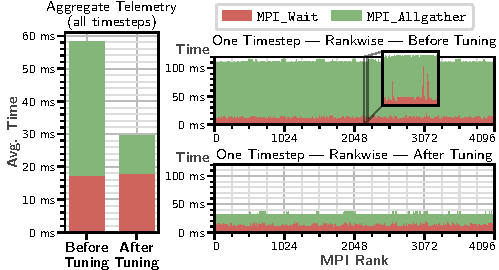
\includegraphics[width=\columnwidth]{data/figs/orca_lesson_volfunc_zoom.pdf}
    \caption{Telemetry from an AMR code where a volatile \mpiw{} precedes \texttt{MPI\_Allgather}.
      Aggregate telemetry (left) misattributes straggler-induced \mpiw{} as elevated collective cost.
      Fine-grained telemetry (right) makes the cause obvious but requires joining all ranks' telemetry.
    }
    \label{fig:orca:bg-volatile}
  \end{figure}%
}

% Fig 5.2: Design: ORCA Architecture
\newcommand{\figDesignArch}{%
  \begin{figure}[t]
    \centering
    
\includegraphics[width=0.8\textwidth, trim=0.2cm 0cm 0.2cm 0cm, clip]{orca-arch.pdf}
    \caption{ORCA architecture.
      A three-tier TBON with application ranks (\tiermpi{}) at the leaves, intermediate aggregators
      (\tieragg{}), and a controller (\tierctl{}) at the root.
      Telemetry originates as columnar timestep dataframes, is transformed by SQL plan operators at each
      tier, and persisted via DuckDB and Parquet sinks --- enabling workflows from real-time feedback via
      lightweight metrics to zero-ETL post-hoc analytics.
    }
    \label{fig:orca:des-arch}
  \end{figure}%
}

% Fig 5.3: Design: ORCA Flow Plan
\newcommand{\figDesignPlan}{%
  \begin{figure}[t]
    \centering
    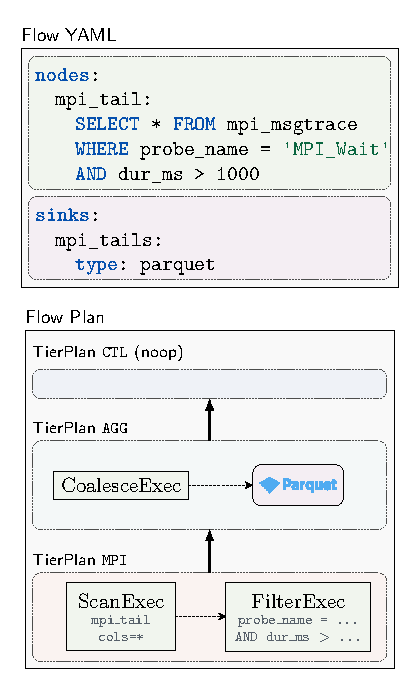
\includegraphics[width=0.4\textwidth, trim=0.35cm 0cm 0.2cm 0.4cm, clip]{data/figs/orca_plan.pdf}%
    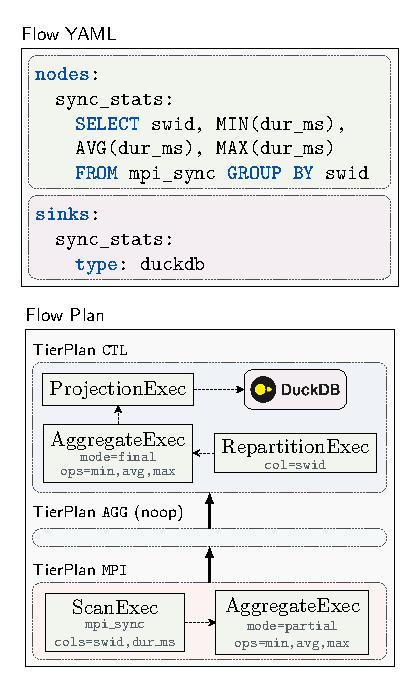
\includegraphics[width=0.4\textwidth, trim=0.3cm 0cm 0.3cm 0.4cm, clip]{data/figs/orca_plan2.pdf}
    \caption{OrcaFlow compilation showing flows and their compiled tier plans.
      Flows chain SQL transforms over telemetry streams en route to configurable sinks.
      Both operators and sinks are placed automatically.
      (Left) A selective filter pushed to \tiermpi{}, discarding most data at source.
      (Right) Aggregations also reduce data volume --- pushed-down partial aggregations emit fixed-size intermediates regardless of input volume.
    }
    \label{fig:orca:des-plan}
  \end{figure}%
}

% Fig 5.4: Design: TS2PC Protocol
\newcommand{\figDesignTwopc}{%
  \begin{figure}[t]
    \centering
    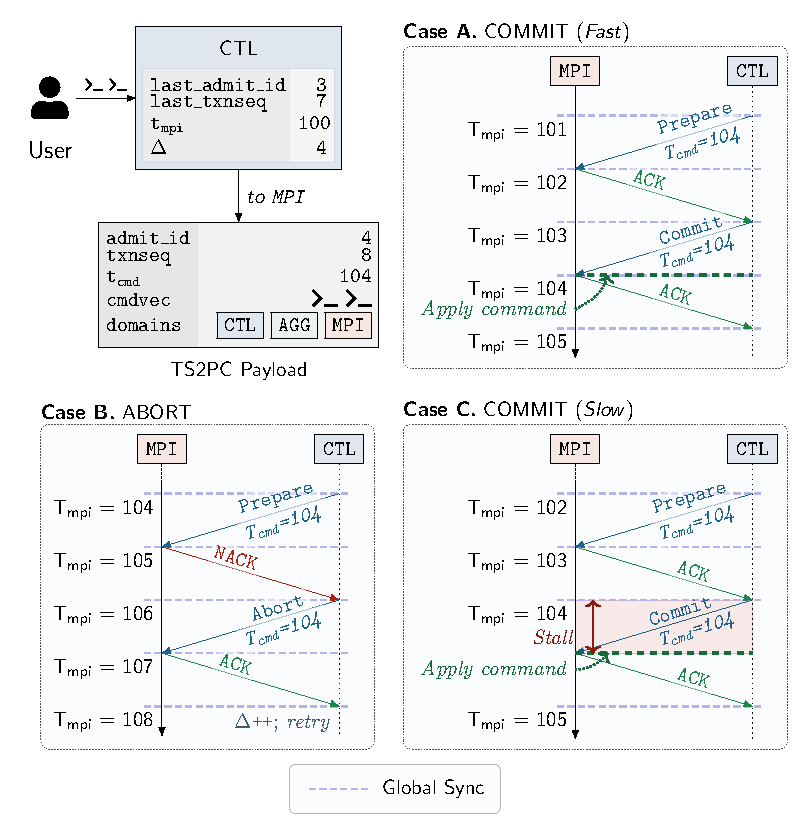
\includegraphics[width=0.8\textwidth, trim=0.2cm 0cm 0.2cm 0cm, clip]{data/figs/orca_ts2pc.pdf}
    \caption{Timestep-linked two-phase commit (\twopc{}).
      Commands are proposed for a future timestep $T_{cmd} = T_{mpi} + \Delta$.
      (A) Normal case: ranks agree and apply the command before executing $T_{cmd}$.
      (B) Abort: ranks have passed $T_{cmd}$ and vote to abort, command is retried with a
      larger $\Delta$. (C) Stall: ranks have prepared but not received commit/abort.
      Execution blocks until resolution to preserve correctness.
    }
    \label{fig:orca:des-twopc}
  \end{figure}%
}

% Fig 5.5: Eval: Runtime overhead, 2x2
\newcommand{\figEvalOverhead}{%
  \begin{figure}[t]
    \centering
    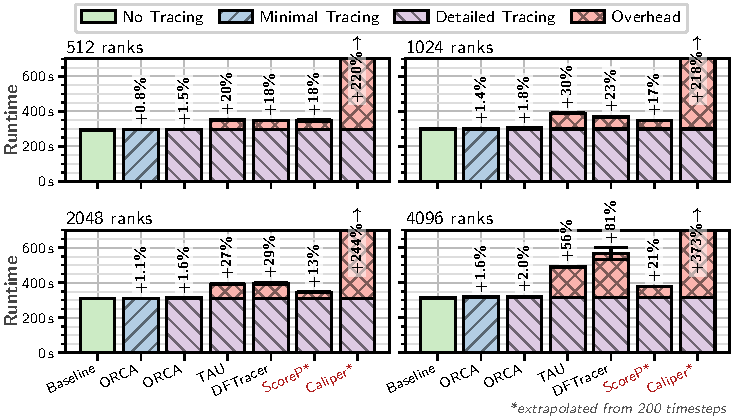
\includegraphics[width=\textwidth]{data/figs/orca_amr_tracer_runtimes_2x2.pdf}
    \caption{Runtime overhead for a detailed tracing profile on an AMR code at 512--4096 ranks.
      An additional minimal profile (collective-only) for ORCA shows always-on overhead.
      ORCA maintains 0.8--2\% overhead across both profiles, while TAU and \dftracer{} degrade from
      18--20\% at 512 ranks to 56--81\% at 4096 ranks.
      \emph{*extrapolated from 200 timesteps due to stability issues.}
    }
    \label{fig:orca:eval-runtime}
  \end{figure}%
}

% Fig 5.6: Eval: Trace size only, one-column
\newcommand{\figEvalSizeOnly}{%
  \begin{figure}[t]
    \centering
    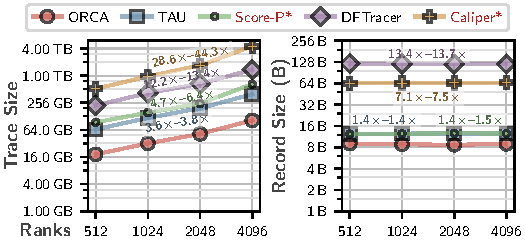
\includegraphics[width=0.8\columnwidth]{data/figs/orca_amr_tracesizes_line.pdf}
    \caption{Trace size (left) and per-record size (right) comparison for detailed profile.
      ORCA traces are 3.6--44$\times$ smaller than other formats.
      Per-record size isolates format efficiency from record amplification --- other tracers emit
      2.5--3.3$\times$ more records than ORCA for the same collection profile.
    }
    \label{fig:orca:eval-tracesize}
  \end{figure}%
}

% Fig 5.7: Eval: Query suite only, one-column
\newcommand{\figEvalQueryOnly}{%
  \begin{figure}[t]
    \centering
    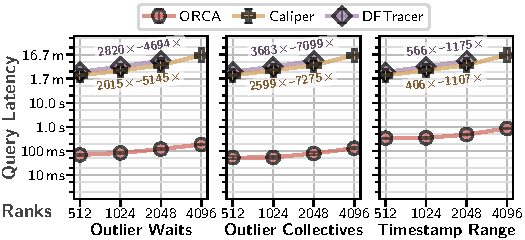
\includegraphics[width=0.8\columnwidth]{data/figs/orca_query_suite_abs.pdf}
    \caption{Post-mortem query performance.
      ORCA completes queries in hundreds of milliseconds, 3--4 orders of magnitude faster than
      \dftracer{} and Caliper.
      Performance for plaintext formats is dominated by parsing, not query complexity.
      TAU and \scorep{} are omitted as OTF2 is not a queryable format.
    }
    \label{fig:orca:eval-query}
  \end{figure}%
}

% Fig 5.8: Eval: Architecture comparison (OFI/TCP + DFTracer compression)
\newcommand{\figEvalArch}{%
  \begin{figure}[t]
    \centering
    \begin{subfigure}[t]{0.64\textwidth}
      \centering
      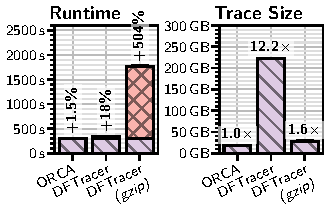
\includegraphics[height=0.22\textheight]{data/figs/orca_dftracer_comp.pdf}
      \caption{Compression impact.}\label{fig:orca:eval-arch-dft}
    \end{subfigure}
    \hfill
    \begin{subfigure}[t]{0.32\textwidth}
      \centering
      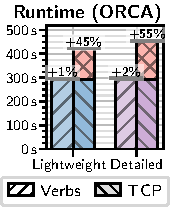
\includegraphics[height=0.22\textheight]{data/figs/orca_ofi_tcp_tracer_runtimes.pdf}
      \caption{Transport impact.}\label{fig:orca:eval-arch-tcp}
    \end{subfigure}
    \caption{(Left) Compression reduces trace size but induces severe jitter on simulation ranks.
      ORCA avoids this by offloading compression to dedicated aggregators.
      (Right) TCP transport increases ORCA overhead from 1--2\% to 45--55\%.
      Arrow-RDMA co-design is essential for low overhead.
    }
    \label{fig:orca:eval-arch}
  \end{figure}%
}

% Fig 5.9: Eval: Online vs offline
\newcommand{\figEvalOrcaNative}{%
  \begin{figure}[t]
    \centering
    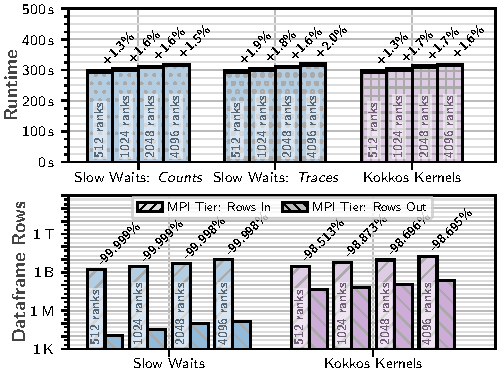
\includegraphics[width=0.8\columnwidth]{data/figs/orca_ontv_combined.pdf}
    \caption{Runtime overhead (top) and MPI tier data reduction (bottom) for in-situ analytics with operator pushdown.
      Flows range from monitoring communication outliers to compute load balance.
      Pushdown discards 98.5--99.999\% of data at sub-2\% overhead, despite operators executing on MPI
      ranks.
    }
    \label{fig:orca:eval-ontv}
  \end{figure}%
}

% Fig 5.10: Eval: Agentic debugging timeline
\newcommand{\figEvalAgentic}{%
  \begin{figure}[t]
    \centering
    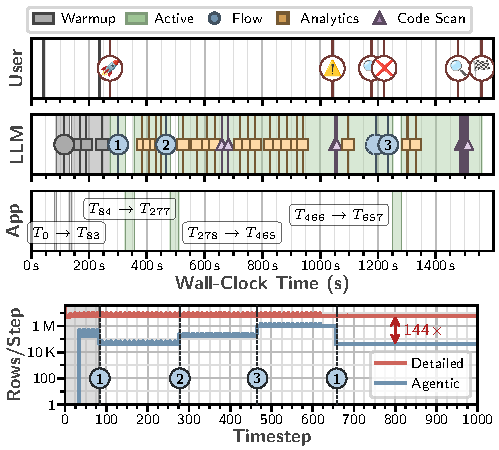
\includegraphics[width=0.8\columnwidth]{data/figs/orca_agentic_timeline.pdf}
    \caption{Visual transcript of an agentic debugging session demonstrating closed-loop capabilities.
      An LLM agent is tasked with localizing the anomaly from \cref{fig:orca:bg-volatile} using high-level
      metrics, progressively collecting targeted telemetry to identify the source.
      The agent operates largely autonomously, producing the complete call path in 27 minutes.
      Reverting to baseline monitoring reduces data volume by 144$\times$.
    }
    \label{fig:orca:eval-agentic}
  \end{figure}%
}

% Table 5.1: Eval: In-situ workflows
\newcommand{\tabEvalFlows}{%
  \begin{table}[t]
    \centering
    \small
    \begin{tabular}
      {@{}p{3cm}p{7.5cm}@{}}
      \toprule
      \textbf{Flow}    & \textbf{Query}                                                                                                \\
      \midrule
      Slow Wait Counts &
      \texttt{SELECT COUNT(*) FROM mpi\_wait WHERE~duration > 1ms} \textcolor{gray}{$\rightarrow$ DuckDB}                              \\
      \addlinespace
      Slow Wait Traces &
      \texttt{SELECT * FROM mpi\_wait WHERE~duration~>~1ms}~\textcolor{gray}{$\rightarrow$ Parquet}                                    \\
      \addlinespace
      Load Imbalance   &
      \texttt{SELECT rank, SUM(duration) FROM kokkos WHERE name IN \textcolor{gray}{<compute kernels>}}                                \\
                       & \texttt{GROUP BY rank} \textcolor{gray}{$\rightarrow$ \texttt{\textcolor[HTML]{B48EAD}{stats}}} \textcolor{gray}{$\rightarrow$ Parquet} \\
                       & \texttt{PERCENTILES(\textcolor[HTML]{B48EAD}{stats}, [50,90,99])} \textcolor{gray}{$\rightarrow$ DuckDB}                                \\
      \bottomrule
    \end{tabular}
    \caption{In-situ workflows evaluated in \Cref{sec:orca:eval-insitu}, ranging from lightweight metrics and selective tracing on the communication path to aggregates over compute kernels.}
    \label{tab:orca:ontv-flows}
  \end{table}%
}
